\section{Quantum chromodynamics}
\label{sec:QCD}

The quantum field theory for the strong interaction, \textit{Quantum Chromodynamics} (\QCD{}), is similar in many ways to that of \QED{}.
The strong interactions are highlighted in red on Fig.\,\ref{fig:feyn-qcd}.
\begin{figure}[h!]
\centering
\begin{tikzpicture}
\begin{feynman}
	\vertex [red!50](i1){\(d\)};
	\vertex [red!50,right=3cm of i1](a);
	\vertex [red!50,above right=0.75cm and 1.5cm of a] (b){ISR};
	\vertex [red!50,below right=0.75cm and 1.5cm of a] (c);

	\vertex [red!50,above=2em of i1](i1a){\(u\)};
	\vertex [red!50,above=1em of i1](i1b){\(u\)};
	\vertex [black!50,right=3cm of i1a](i1ai);
	\vertex [black!50,right=3cm of i1b](i1bi);
	\vertex [black!50,above right=0.75cm and 1.5cm of i1ai] (i1aii);
	\vertex [black!50,above right=0.75cm and 1.5cm of i1bi] (i1bii);

	\vertex [right=1cm of i1a](g1);
	\vertex [right=2cm of i1a](g2);

	\vertex [red!50,below=5em of i1](i2){\(u\)};
	\vertex [red!50,right=1.5cm of i2] (d);
	\vertex [red!50,above right=0.75cm and 1.5cm of d] (e);
	\vertex [red!50,below right=0.75cm and 1.5cm of d] (f);
	\vertex [red!50,below right=0.75cm and 1.5cm of e] (g);
	\vertex [red!50,above right=0.75cm and 1.5cm of e] (h);

	\vertex [red!50,below=1em of i2](i2a){\(u\)};
	\vertex [red!50,below=2em of i2](i2b){\(d\)};
	\vertex [black!50,right=1.5cm of i2a](i2ai);
	\vertex [black!50,right=1.5cm of i2b](i2bi);
	\vertex [black!50,below right=0.75cm and 1.5cm of i2ai] (i2aii);
	\vertex [black!50,below right=0.75cm and 1.5cm of i2bi] (i2bii);

	\vertex [red!50,right=2cm of h] (i);
	\vertex [red!50,above right=1.5cm and 1.5cm of i] (j);
	\vertex [red!50,below right=1.5cm and 1.5cm of i] (k);
	\vertex [red!50,above right=1.2cm and 1.5cm of j] (j1);
	\vertex [red!50,below right=1.2cm and 1.5cm of j] (j2);
	\vertex [red!50,above right=1.2cm and 1.5cm of k] (k1);
	\vertex [red!50,below right=1.2cm and 1.5cm of k] (k2);

	\vertex [black!50,above right=0.5cm and 1.5cm of j1] (l1){\(\ell\)};
	\vertex [black!50,below right=0.5cm and 1.5cm of j1] (l2){\(\overline \nu_\ell\)};
	\vertex [black!50,above right=0.5cm and 1.5cm of k1] (m1){\(q\)};
	\vertex [black!50,below right=0.5cm and 1.5cm of k1] (m2){\(\overline q'\)};
	\vertex [red!50,above right=0.5cm and 1.5cm of k2] (o1){\(\overline b\)};
	\vertex [red!50,below right=0.5cm and 1.5cm of k2] (o2){FSR};

	\diagram* {
	(i1) -- [red!50,fermion] (a) -- [red!50,fermion, edge label=\(q\)] (h),
	(g1) -- [red!50,gluon, half left] (g2),
	(a) -- [red!50,gluon] (b),
	(i2) -- [red!50,fermion] (d) -- [red!50,gluon] (e),
	(d) -- [red!50,fermion] (f),
	(e) -- [red!50,fermion] (g),
	(h) -- [red!50,fermion, edge label=\(\overline q\)] (e),
	(h) -- [very thick,red,gluon] (i),
	(i) -- [very thick,red,fermion, edge label=\(t\)] (j),
	(k) -- [very thick,red,fermion, edge label=\(\overline t\)] (i),
	(j) -- [black!50,boson, edge label=\(W^+\)] (j1),
	(j) -- [black!50,fermion, edge label=\(b\)] (j2),
	(k) -- [black!50,boson, edge label=\(W^-\)] (k1),
	(k2) -- [red!50,fermion, edge label=\(\overline b\)] (k),
	(j1) -- [black!50,fermion] (l1),
	(l2) -- [black!50,fermion] (j1),
	(k1) -- [black!50,fermion] (m1),
	(m2) -- [black!50,fermion] (k1),
	(o1) -- [red!50,fermion] (k2),
	(k2) -- [red!50,gluon] (o2),
	(i1a) -- [red!50,fermion] (i1ai) -- [red!50,fermion] (i1aii),
	(i1b) -- [red!50,fermion] (i1bi) -- [red!50,fermion] (i1bii),
	(i2a) -- [red!50,fermion] (i2ai) -- [red!50,fermion] (i2aii),
	(i2b) -- [red!50,fermion] (i2bi) -- [red!50,fermion] (i2bii),
	};
\end{feynman}
\end{tikzpicture}
\caption[A Feynman diagram showing the \ttbar{} pair production and decay. An example QCD interaction is shown in bold red. Other QCD interactions are shown in light red.]{A Feynman diagram showing the \ttbar{} pair production and decay. An example QCD interaction is shown in bold red. Other QCD interactions are shown in light red.}
\label{fig:feyn-qcd}
\end{figure}
It is described by an $\mathrm{SU(3)}$ symmetry group, with three orthogonal states known as colour charges ($r,g,b$).
To maintain invariance under the local $\mathrm{SU(3)}$ gauge transformation,
\begin{equation}
\Psi(x) \to e^{i\theta^{a}(x)t^{a}}\Psi(x),
\end{equation}
eight new gauge fields, $G_{\mu}^{a}$, must be introduced in a similar manner to \QED{}.
These fields come from the eight generators of the $\mathrm{SU(3)}$ symmetry group $t^{a}$, which are related to the Gell-Mann matrices by $t^{a}=-\frac{1}{2}\lambda^{a}$.
As with \QED{}, the extra fields are folded into the covariant derivative, this time with a strong coupling constant $g_{s}$
\begin{equation}
D_{\mu} = \partial_{\mu}+ig_{s}\frac{\lambda_{a}}{2}G_{\mu}^{a}.
\end{equation}
Thus the strong force is mediated by eight massless gauge bosons (gluons), however, in difference to \QED{}, these gluons carry a colour charge brought about by the non-commutation of the $\mathrm{SU(3)}$ generators, leading to gluon-gluon self-interactions.
The full \QCD{} Lagrangian density is given as
\begin{equation}
\Lagr_{\QCD}=\overline{\Psi}_{i}(i(\gamma^{\mu}D_{\mu})_{ij}-m\delta_{ij})\Psi_{j} - \frac{1}{4}G^{\mu \nu}_{a}G^{a}_{\mu \nu},
\end{equation}
where the gluon field strength tensor, 
\begin{equation}
	G_{\mu \nu}^{a}=\partial_{\mu}G_{\nu}^{a} - \partial_{\nu}G_{\mu}^{a} + g_{s}f^{abc}G_{\mu}^{b}G_{\nu }^{c}
\end{equation}
is analogous to the electromagnetic field strength tensor, with $f^{abc}$ being the $\mathrm{SU(3)}$ fine structure constants.

\subsection{Colour confinement and hadronisation} % (fold)
\label{sub:confinement}
In Fig\,\ref{fig:alphaSrunning}, the running of the strong coupling constant with energy is shown.
\begin{figure}[h!]
	\centering
	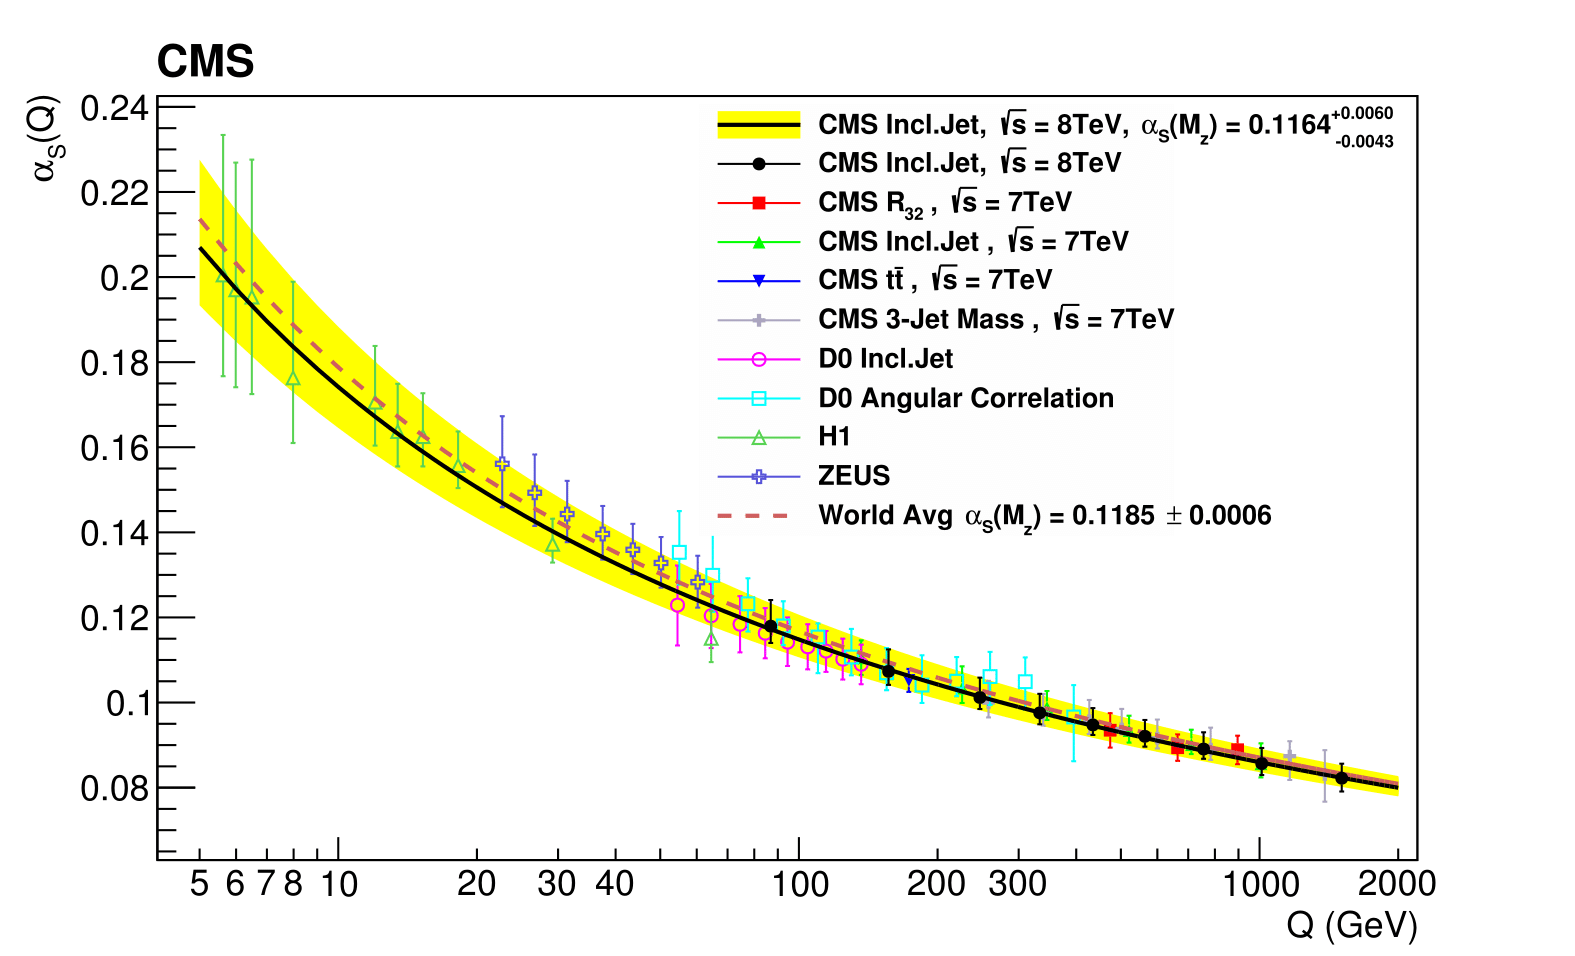
\includegraphics[width=\textwidth]{Figures/alphaS}
	\caption[The running of the strong coupling constant]{The running of the strong coupling constant \cite{alphaSrunning}.}
	\label{fig:alphaSrunning}
\end{figure}
At higher energies $g_{s}$, which is also commonly known as \alpS{}, tends to 0.
This is known as asymptotic freedom and means that the strong force becomes stronger at larger quark or gluon separations.
The quarks and gluons are consequently bound in colourless states (hadrons and mesons) in a process known as \textit{colour confinement}.
Single quarks in the final state of Fig\,\ref{fig:feyn-eg} immeadiately bind into baryons.
These particles can be highly energetic, causing the constituent quarks to strain against each other.
If the potential energy due to the strong force confining the quarks is large enough then a new \qqbar{} pair will be produced from the vacuum. 
If the new daughter hadrons produced have enough energy, they split again until the confinement is strong enough to hold them together.
The splitting of hadrons and mesons in this way is known as \textit{hadronisation} and results in a spray of particles in the final state known in experimental terms as a \textit{jet}.
Similarly, when a hard interaction occurs within the colliding protons, the protons cease to become colourless states, and the remnants hadronise forming more sprays of particles.
These particles are known as the \textit{underlying event}.
The hadronisation process will be discussed in more detail in Section TODO.
% subsection confinement (end)
